\chapter{The Standard Model}
\label{sec:standardModel}
\begin{quote}
  A possible explanation of the physicist's use of mathematics to formulate his laws of nature is that he is a somewhat irresponsible person.\\ \quotebox{\hfill - Eugene Wigner}
\end{quote}

The Standard Model (SM) of particle physics is a relativistic quantum field theory that describes the fundamental particles of matter and their interactions via the electromagnetic, weak nuclear, and strong nuclear forces. The first steps toward the formalization of the SM were taken in the 1960s by the work of Glashow\cite{Glashow:1961tr}, Weinberg\cite{Weinberg:1967tq}, and Salam\cite{Salam:1968rm} that described the unification of the electromagnetic and weak nuclear forces. The SM consists of particles with half integer spin called fermions and particles with integer spin called bosons. All known matter is constructed from the fermionic particles while the bosonic particles are responsible for mediating the interactions between particles. Fermions come in two types -- leptons and quarks -- which are further organized by mass into three generations\footnote{Each generation consists of one left-handed quark doublet, two right-handed quark singlets, a left-handed lepton doublet, and one right-handed charged lepton singlet. There is no current experimental evidence for right handed neutrinos.\cite{Langacker, Rolnick}}. 

The fermions possess various ``charges'' that determine the possible interactions between particles. If a fermion interacts with other particles via a given force, it is said to be ``charged'' under that force and the associated field. Interactions between two fermions charged under the same field proceed via the exchange of the force-carrying bosons. A simple example of this is the Coulomb repulsion between two electrons -- electrons are both charged under the electromagnetic force ($q=-e$) and interact via the exchange of the force-carrying boson of the electromagnetic force, the photon. 
\begin{figure}[!ht]
\centering
\includegraphics[height=1.5in]{figures/standardModel/feynman_coulombInteraction}
\caption{A Feynman diagram depicting the electromagnetic interaction between two electrons. The interaction is mediated by the exchange of a photon (a spin-1 gauge boson).}
\label{feynman}
\end{figure}
A Feynman diagram depicting this interaction is shown in Fig. \ref{feynman}. Figure \ref{periodic} summarizes the particles of the Standard Model as well as some of their fundamental properties like mass, spin, and electric charge. 
\begin{figure}
\centering
\includegraphics[height=3in]{figures/standardModel/SMperiodic}
\caption{The constituents of the Standard Model and their masses, electric charges, and spin information.}
\label{periodic}
\end{figure}
While the charge of the electromagnetic force is electric charge and the mediating boson is the massless photon, the weak nuclear force is mediated by the exchange of heavy $W^{\pm}$ and $Z$ bosons for particles possessing a weak charge, and the strong nuclear force is mediated by the exchange of massless gluons between particles possessing color charge. Charged leptons (unsurprisingly) possess electric charge as well as weak charge while the neutral leptons (neutrinos) possess only a weak charge. Quarks are charged under the electromagnetic, weak, and strong nuclear forces and are the only fermions that interact via the strong force. Figure \ref{interactionsSM} shows a schematic representation of all the particles of the Standard Model and sketches out the allowed interactions between those particles through their connecting lines.
\begin{figure}[!h]
\centering
\includegraphics[height=3in]{figures/standardModel/Elementary_particle_interactions}
\caption{A schematic representation of the Standard Model. All constituent particles are represented by the black circles/ovals while their allowed interactions are signified by the connecting blue lines.}
\label{interactionsSM}
\end{figure}

Gluons can be identified as the gauge fields, $G_i (i=1\cdots8)$, of an $SU(3)$ gauge group. The strong force is non-chiral (i.e. treats right and left handed particles equally), and the $SU(3)$ operators act on the color indices of both left and right handed quarks. An important property of the strong force (also called quantum chromodynamics or QCD) is the confinement of color charge into color singlets. Colored objects (quarks and gluons) cannot exist in isolation, and they quickly hadronize (cascading decays of quarks via the strong force into mesons and baryons) into groups of particles called jets~\cite{Green, HiggsHunter}.

The weak nuclear force and electromagnetism can be combined into an $SU(2)\otimes U(1)$ gauge group~\cite{Weinberg:1967tq}. In contrast to the strong force, the weak force is chiral and acts on the flavor indices of only left handed fermions. The $U(1)$ subgroup is also chiral but acts on both left and right handed fermions~\cite{Rolnick}. The three gauge fields of $SU(2)$, $W_i (i=1,2,3)$, along with the single gauge field of $U(1)$, $B$, combine after electroweak symmetry breaking to form the $W^\pm$, $Z$, and $\gamma$.

The full, unbroken group structure of the Standard Model is written
\begin{equation}
SU(3)_C\otimes SU(2)_L\otimes U(1)_Y
\end{equation}
where the subscripts have physical rather than group significance. $C$ denotes the strong color interaction group, $Y$ represents the weak hypercharge, and $L$ signifies the left-handed nature of the weak force. The full Lagrangian density of the Standard Model can be expressed as the sum
\begin{equation}
\mathcal{L} = \mathcal{L}_{gauge} + \mathcal{L}_{fermion} + \mathcal{L}_{\phi} + \mathcal{L}_{Yukawa}
\end{equation}
where the individual parts refer to the gauge, fermion, Higgs, and Yukawa sectors of the SM. The Yukawa sector describes interactions between scalar and Dirac fields, e.g. flavor changing interactions between quarks via the weak force. The generation of mass for fermions via interaction with the Higgs field is also described by a Yukawa interaction.
\section{Electroweak Theory}
The unification of the weak and electromagnetic force into an $SU(2)_L\otimes U(1)_Y$ gauge group was first accomplished by Glashow~\cite{Glashow:1961tr}. The $SU(2)$ subgroup contains three gauge fields -- one positively charged, one negatively charged, and one neutral. Since the weak interaction is observed to exhibit only a $V-A$ (vector - axial) coupling, only left handed operators are generated by the $SU(2)$ group, hence the $L$ subscript. Right handed fermions are invariant singlets under $SU(2)_L$. Electromagnetism does not discriminate based on handedness, so the neutral field of $SU(2)$ cannot be the photon.

To incorporate the photon, the weak group is enlarged to $SU(2)_L\otimes U(1)_Y$ by adding the independent unitary group, $U(1)_Y$. The conserved quantity associated with this new group is called weak hypercharge and is denoted by the subscript $Y$. The hypercharge operator is defined as $\frac{Y}{2}=Q-I_3$ where $Q$ is the electric charge, and $I_3$ is the third component of weak isospin.

To maintain local gauge invariance under group transformations, the ordinary derivative operator is replaced with the covariant derivative
\begin{equation}\label{covariant}
\partial_\mu\rightarrow D_\mu=\partial_\mu-ig_1\frac{Y}{2}B_\mu-ig_2\left(\frac{\vec{\tau}}{2}\cdot \vec{W_\mu} \right)
\end{equation}
where $\tau_i$'s are the Pauli matrices. The subscript index, $\mu$, signifies the four-vector nature of the relevant objects and runs over the four spacetime dimensions. Inserting the covariant derivative into the %fermion interaction terms ($\sim i\bar\psi_f\gamma^{\mu}D_{\mu}\psi_f$) of the 
SM Lagrangian couples the leptons and quarks to the electroweak gauge fields. The resulting interactions can be grouped into charged current and neutral current interactions with gauge fields~\cite{Rolnick, HiggsHunter}
\begin{equation}
W_{\mu}^{\pm}=\frac{1}{\sqrt{2}}(W_{1\mu}\pm iW_{2\mu}), \,Z^0_{\mu}=\frac{-g_1B_{\mu}+g_2W_{3\mu}}{\sqrt{g_1^2+g_2^2}}
\end{equation}
The neutral field, $Z^0_{\mu}$, cannot be the electromagnetic field, $A_{\mu}$, since it mediates a coupling between left handed neutrinos, electrically uncharged fermions that do not interact electromagnetically. Since $A_{\mu}$ cannot couple to neutrinos, it must be orthogonal to the weak current that does. The gauge fields of $SU(2)_L$ and $U(1)_Y$ are orthogonal by construction, so the weakly orthogonal electromagnetic gauge field is defined
\begin{equation}
A_{\mu}=\frac{g_2B_{\mu}+g_1W_{3\mu}}{\sqrt{g_1^2+g_2^2}}
\end{equation}

The extended electroweak gauge group provides the structure to accommodate the electromagnetic and weak forces, but the extremely short range of the weak force ($\mathcal{O}$(1 fm)) remains problematic. A gauge group exhibiting an exact symmetry, such as quantum electrodynamics (QED), contains massless gauge fields which mediate a force with infinite extent. The short range of the weak force implies massive mediating gauge fields; however, mass terms cannot be added directly to the SM Lagrangian while maintaining gauge invariance. In order to reproduce observed physical phenomena, current theory holds that the $SU(2)_L\otimes U(1)_Y$ symmetry of the Standard Model must be spontaneously broken.
\section{Higgs Mechanism}
The Englert-Brout-Higgs-Guralnik-Hagen-Kibble mechanism, proposed in the early 1960s by several independent groups~\cite{PhysRevLett.13.508, PhysRevLett.13.321, PhysRevLett.13.585} and often called simply the Higgs mechanism, is one way to generate the required symmetry breaking. This spontaneous symmetry breaking (SSB) can be accomplished by the introduction of a complex scalar doublet field
\begin{equation}\label{doublet}
\phi = 
\begin{pmatrix}
\phi^+\\\phi^0
\end{pmatrix}
\end{equation}
where the superscripts denote electric charge. The Lagrangian for such a field is written as
\begin{equation}
\mathcal{L}_{\phi}=T-V=\left(\partial_{\mu}\phi\right)^{\dagger}\left(\partial^{\mu}\phi\right)-\mu^2\phi^{\dagger}\phi-\lambda(\phi^{\dagger}\phi)^2
\label{eq:higgsLagrangian}
\end{equation}
where $V=\mu^2\phi^{\dagger}\phi+\lambda(\phi^{\dagger}\phi)^2$ is the potential and $\mu^2 < 0$. The complex fields in Eq. \ref{doublet} can be rewritten in terms of real fields $\phi^+=(\phi_1+i\phi_2)/\sqrt{2}$ and $\phi^0=(\phi_3+i\phi_4)/\sqrt{2}$, yielding
\begin{equation}\label{eq:lagrange2}
\mathcal{L}=\frac{1}{2}\sum^4_{i=1}(\partial^\mu\phi_i)(\partial_\mu\phi_i)-\frac{\mu^2}{2}\sum^4_{i=1}\phi_i\phi_i-\frac{\lambda}{4}\left(\sum^4_{i=1}\phi_i\phi_i\right)^2
\end{equation} 
which is invariant under a global $SO(4)$ phase rotation in $\phi$-space. If $\mu^2$ is positive, the potential has a minimum at $\Phi^2=(\phi_1+\phi_2+\phi_3+\phi_4)^2=0$, and the $SO(4)$ symmetry remains unbroken. However, if $\mu^2 < 0$, the potential is minimized around a circle with radius $v=\sqrt{\frac{-\mu^2}{\lambda}}$. The vacua of the field can be arbitrarily rotated such that $\phi_1=\phi_2=\phi_4=0$, yielding vacuum expectation values (VEVs) of $\Braket{0|\phi^0|0}=\frac{v}{\sqrt{2}}, \Braket{0|\phi^+|0}=0$.

After breaking and rotation, the Higgs doublet is written
\begin{equation}\label{broken}
\phi = \frac{1}{\sqrt{2}}
\begin{pmatrix}
0\\v+h(x)
\end{pmatrix}
\end{equation}
This new field, $h(x)$ is identified as the physical Higgs boson.\cite{PhysRevLett.13.508, PhysRevLett.13.321, PhysRevLett.13.585}

The weak gauge bosons gain mass through interactions arising from the covariant derivatives in the kinetic portion of Eq. \ref{eq:lagrange2}. Inserting the covariant derivatives and keeping terms proportional to the square of the gauge fields yields
\begin{equation}
(D_{\mu}\phi)^{\dagger}(D^{\mu}\phi)_{mass}\sim(\frac{vg_2}{2})^2W^{+\dagger\mu}W^{-\dagger}_{\mu}+\frac{1}{2}(\frac{v\sqrt{g_1^2+g_2^2}}{2})^2Z^{\mu}Z_{\mu}
\end{equation}
The masses of the gauge bosons are thus identified as
\begin{equation}
m_W=\frac{vg_2}{2},\,\,m_Z=\frac{v\sqrt{g_1^2+g_2^2}}{2},\,\,m_A=0
\end{equation}

The electromagnetic field $A_\mu$ remains massless since no corresponding term is generated in the symmetry breaking. Electromagnetic charge conservation is also preserved. SSB breaks the extended electroweak group into the $U(1)$ gauge group of QED and the $SU(3)_C$ color group of QCD:  
\begin{equation}
SU(3)_C\otimes SU(2)_L\otimes U(1)_Y \rightarrow SU(3)_C\otimes U(1)_{QED}
\end{equation}
Mass terms for fundamental fermions can be generated by the Higgs mechanism via a Yukawa coupling between left and right handed fermions and the Higgs field. The SM Higgs is also required to be a spin-0 (scalar) boson even under charge-parity (CP) conjugation~\cite{Carena:577783}. 

\subsection{Single Higgs Production}
Single Higgs boson production can occur via four different processes
\begin{itemize}
\item gluon-gluon fusion (ggF)
\item vector boson fusion (VBF)
\item vector boson associated production (VH)
\item \ttbar associated production ($ttH$)
\end{itemize}
The leading order Feynman diagrams for each process are shown in Figure~\ref{fig:higgsProductionFeynman}.
\begin{figure}[h!]
\centering
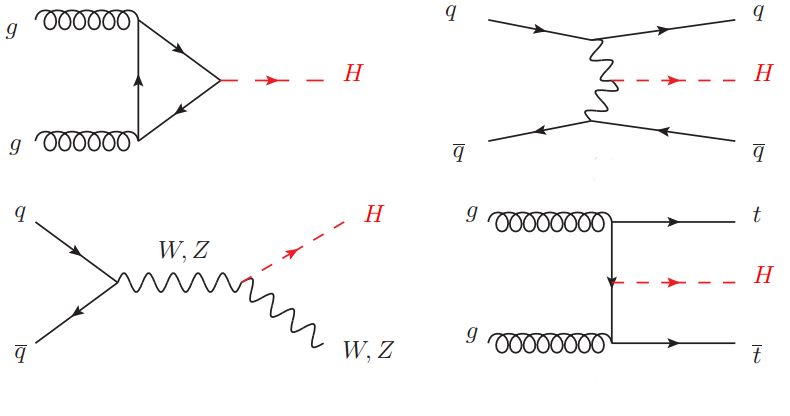
\includegraphics[height=3in]{figures/standardModel/higgs_prod_mech_pdg}
\caption{Feynman diagrams for single Higgs boson production via the a) gluon fusion, b) vector boson fusion, c) association with a vector boson, and d) association with a \ttbar pair.}
\label{fig:higgsProductionFeynman}
\end{figure}

Since hadronic accelerators do not collide individual quarks or gluons but rather hadrons such as protons, the rate of each production mechanism is set by the relative abundance of quarks, anti-quarks, and gluons in the colliding hadrons. Probability distributions called parton distribution functions (PDFs) are produced using measurements from fixed target and collider experiments~\cite{mstw1, mstw2, Lai:2010vv, ct102, nnpdf, ref:pdf4lhc} and model the probability for a particle of species $s$ inside a hadron (e.g. a proton or anti-proton) to possess a given fraction, $x$, of the total momentum of the hadron. The more abundant a particle is at relatively low fractional energy, the more likely it is that for that particle to be involved in a collision with another hadron. Figure~\ref{fig:mstwPDF} shows the parton distribution functions obtained by the MSTW collaboration~\cite{mstw1}. 
\begin{figure}[h!]
\centering
\includegraphics[height=3.0in]{figures/standardModel/mstw2008_cl68_pdfDistributions}
\caption{Parton distribution functions developed by the MSTW collaboration for the gluons and quarks (up/down/strange/charm/bottom) found in protons. The x-axis is represents the fractional momentum possessed by a particle inside the proton and the y-axis is the fractional momentum times population frequency as a function of fractional momentum and momentum transfer.}
\label{fig:mstwPDF}
\end{figure}
At a proton-proton collider like the LHC, the gluon fusion production mechanism is dominant due to the relatively large population of gluons with enough combined energy to produce a Higgs boson. Figure~\ref{fig:higgsProductionRates} shows the rates of each production mechanism for a $pp$ collider like the LHC.

\begin{figure}[h!]
\centering
\includegraphics[height=3.5in]{figures/standardModel/higgsProductionRates}
\caption{Standard Model Higgs production rates as a function of center of mass energy.}
\label{fig:higgsProductionRates}
\end{figure}

As gluons do not couple directly to the Higgs boson (gluons are perturbatively massless), the gluon fusion diagram proceeds via a quark loop interaction which couples directly to the Higgs field through its Yukawa coupling. Since the Higgs-fermion Yukawa couplings are directly proportional to the fermion mass, the contribution from the top quark loop dominates the gluon fusion mode. For a Higgs mass of 125 GeV, the cross-section for the gluon fusion production mechanism at the LHC is $\sigma_{\text{ggF}} = $19.27 pb$^{-1}$ at $\sqrt{s} = $8 TeV and 43.92 pb$^{-1}$ at $\sqrt{s} = $13 TeV~\cite{Heinemeyer:2013tqa}. While the gluon fusion mode has the largest cross-section at the LHC, the lack of additional identifying features (e.g. no associated jets or leptons produced in the interaction) makes for larger backgrounds relative to other production modes. Still, the larger cross-section of the gluon fusion mode means this is a dominant mode for analysis at the LHC.

In production via vector boson fusion, an incoming quark and anti-quark pair scatter off each other via the exchange of $W$ or $Z$ bosons, and the resulting vector bosons fuse to produce a Higgs boson. The outgoing quarks pick up a large recoil from the emission of the heavy $W/Z$ bosons, and the final state for vector boson production is characterized by the presence of two high momentum quark jets in addition to the decay products of the Higgs itself. While the cross-section for Higgs production via the vector boson fusion mode is small at the LHC for a Higgs with a mass of 125 GeV ($\sigma_{\text{VBF}} = $1.58 pb$^{-1}$ at $\sqrt{s} = $8 TeV, 3.75 pb$^{-1}$ at $\sqrt{s} = $13 TeV~\cite{Heinemeyer:2013tqa}), the VBF mode has a higher signal to background ratio compared to the gluon fusion mode after requiring the presence of two high momentum jets in addition to the Higgs in the final state.

The associated production (VH) mode is characterized by the production of a Higgs boson in association with a $W$ or $Z$ vector boson. In this process, the heavy vector boson is produced via quark/anti-quark annihilation and radiates a Higgs boson before decaying to either leptons or quarks. In analogy with the bremsstrahlung process by which an electrically charged particle emits a photon, the associated production mechanism is often also referred to as higgsstrahlung. For a Higgs mass of 125 GeV, the cross-section for the associated production mechanism at the LHC is $\sigma_{\text{VH}} = $1.12 pb$^{-1}$ at $\sqrt{s} = $8 TeV and 2.25 pb$^{-1}$ at $\sqrt{s} = $13 TeV~\cite{Heinemeyer:2013tqa}. The presence of the high \pt decay products of the $W/Z$ boson in the final state (especially for leptonic decays) is a powerful handle for reducing backgrounds despite the relatively low cross-section.

The last mode for single Higgs production at the LHC is the production of a Higgs boson in association with a pair of top quarks (also referred to as the \ttH mode). The \ttH mode can be proceed via the collision of two gluons that produce a top quark/anti-quark pair of which one quark radiates a Higgs boson (this diagram is shown in Fig.~\ref{fig:higgsProductionFeynman}). The \ttH mode can also be produced from the fusion of two gluons into a single gluon which then splits into a top quark/anti-quark pair of which one top radiates a Higgs. The presence of the \ttbar pairs in addition to the Higgs boson gives the \ttH production mode a rich final-state phenomenology, but the low cross sections ($\sigma_{\ttH} = $0.13 pb$^{-1}$ at $\sqrt{s} = $8 TeV and 0.51 pb$^{-1}$ at $\sqrt{s} = $13 TeV~\cite{Heinemeyer:2013tqa} for a 125 GeV Higgs) make this a challenging process to search for at the LHC.

\subsection{Single Higgs Decay}
\label{sec:higgsDecay}
Once produced, the Higgs boson can decay into a particle/anti-particle pair of any particle coupling to the Higgs field via mass. Since the Higgs-fermion coupling is proportional to the fermion mass and the Higgs-boson coupling is proportional to the boson mass squared, the larger the mass of a particle coupled to the Higgs, the larger the branching fraction of Higgs decays. Figure~\ref{fig:higgsBranchingFractions} shows the Higgs branching fractions as a function of mass~\cite{Dittmaier:2011ti}. Decays to final states of massless particles, e.g. pairs of photons or gluons, proceeds via a quark or heavy vector boson loop analogous to the loop in gluon fusion production shown in in Fig.~\ref{fig:higgsProductionFeynman}.

\begin{figure}[h!]
\centering
\includegraphics[width=.6\textwidth]{figures/standardModel/higgsXS_BR_125}
\caption{Standard Model branching fractions for a Standard Model Higgs across a range of Higgs masses. The black line vertical line at 125 GeV shows the branching fractions for the Higgs boson measured by the ATLAS and CMS collaborations.}
\label{fig:higgsBranchingFractions}
\end{figure}

The branching fractions depend strongly on the mass of the Higgs, and for the observed Higgs mass of 125.09 $\pm$ 0.24 GeV~\cite{Aad:2015zhl}, the $b\bar{b}$ and $WW^*$ decay modes have the largest branching fractions, accounting for 79.3\% of all Higgs decays~\cite{Heinemeyer:2013tqa}. While other modes such as $\gamma\gamma$ and $ZZ^*$ have relatively smaller branching fractions (0.23\% and 2.67\% respectively), searches for these decay modes can yield more sensitive (larger ratio of signal to background events) results compared to decay modes with larger branching fraction due to their relatively smaller Standard Model backgrounds. The $h\rightarrow ZZ^*$ in the fully leptonic decay channel in particular has enormous sensitivity since the SM 4$\ell$ background is tiny. Combining measurements of Higgs properties in multiple decay channels improves the overall precision of our knowledge about the Higgs boson and the mechanism behind electroweak symmetry breaking.

\subsection{Double Higgs Production}
While single Higgs production can occur via a number of processes, Higgs bosons can also be produced in pairs through Higgs self-interactions or via double higgsstrahlung. Probing the Higgs self-interactions explores a completely new sector of physics and has great potential (pun not intended) for the field of precision Higgs measurements. The potential of the Lagrangian in Eq.~\ref{eq:lagrange2} has a minimum at $\phi = \pm \sqrt{\frac{-\mu^2}{\lambda}}$. Taking $\phi$ to be a simple scalar field as an example, we can introduce the field variable
\begin{equation}
\eta = \phi \pm \sqrt{\frac{-\mu^2}{\lambda}}
\end{equation}
the Lagrangian in Eq.~\ref{eq:lagrange2} becomes
\begin{equation}
\mathcal{L}_{\phi}=\frac{1}{2}\left(\partial_{\mu}\eta\right)\left(\partial^{\mu}\eta\right)-\mu^2\eta^2 \pm \mu\lambda\eta^3 - \frac{1}{4}\lambda^2\eta^4 + \frac{1}{4}(\mu^2/\lambda)^2
\label{eq:higgsLagrangian2}
\end{equation}
The first two terms are the familiar kinetic and mass terms, but now we have additional terms proportional to $\eta^3$ and $\eta^4$. These terms represent self-couplings of the Higgs field of the third and fourth order. Eqs~\ref{eq:lagrange2} and ~\ref{eq:higgsLagrangian2} describe identical physics, but the second formulation presents the self-interactions in more evident way. Diagrams for the leading order ($\sim\eta^3$) Higgs self-interaction and double higgsstrahlung (via a quark loop and quark-Higgs Yukawa couplings) are shown in Fig.~\ref{fig:SM-dihiggs-prod}.
\begin{figure}[h!]
\centering
\label{fig:SM-dihiggs-prod}
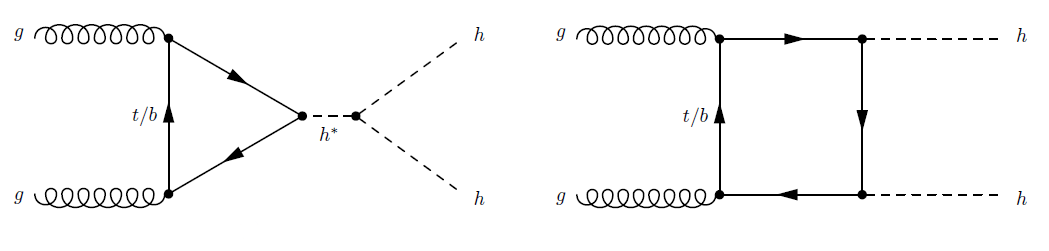
\includegraphics[width=.8\textwidth]{figures/standardModel/SM-diHiggs-production}
\caption{Leading order Feynman diagrams for dihiggs production due to a) the Higgs self-interaction and b) the Higgs-fermion Yukawa interaction.}
\end{figure}

The Standard Model contributes to dihiggs production only through non-resonant modes, but many models of new physics can yield additional contributions to dihiggs production when that new physics couples to the SM Higgs sector~\cite{Dolan:2012ac}. In the minimal supersymmetric extension of the Standard Model (the MSSM), there are five Higgs bosons (one neutral light CP even, one neutral heavy CP even, one neutral CP odd, and two charged Higgs bosons) of which the neutral light CP even Higgs, $h$, can be identified as the Standard Model Higgs boson. The heavy neutral CP even Higgs, $H$, can decay into $hh$ pairs due to the mixing of the Higgs doublets in the model. Measuring the rate of dihiggs production in this context can then be used to constrain the range of possible masses and mixing angles in the theory. Figure~\ref{fig:BSM-dihiggs-prod} shows a leading order example of an $H$ resonance decaying to two Higgs bosons. %In the context of the MSSM, this $X$ can be identified as the heavy, neutral component of the second Higgs doublet. CHECK THAT.
\begin{figure}[h!]
\centering
\label{fig:BSM-dihiggs-prod}
\includegraphics[width=.35\textwidth]{figures/standardModel/BSM-dihiggs-prod_W}
\caption{Schematic Feynman diagram showing gluon fusion initiated production of an exotic resonance, $H$, and its decay into two Higgs bosons.}
\end{figure}

\section{Top Physics}
The top quark, discovered in 1995 by the D0 and CDF collaborations at Fermilab~\cite{CDF, D0}, is the heaviest particle in the SM. Top quarks decay nearly universally via $t\rightarrow Wb$ and have a lifetime of $\sim 10^{-25}$ seconds. % which can be expressed analytically as 
%\begin{equation}
%\label{eq:topQuarkLifetime}
%\tau_{\text{top}}= \frac{\mid V_{tb}\mid}{m_t^2}
%\end{equation}
The top is so massive that its lifetime is much smaller than the time it would take to hadronize ($\sim 10^{-23}$ s), so precision measurements of top quark decays allow for measurements of the `bare' electroweak properties of the top quark. Studying distributions sensitive to the production mechanisms of top quarks allows for constraints on PDF, and studying the high energy tails of top quark distributions acts as a probe of the existence of any new physics coupling to the Standard Model via mass. In short, precision top quark measurements can help say a lot about how high energy physics works at the edge of our understanding.

\subsection{Top Quark Production}
Top quarks can be produced in a variety of ways, and at a hadron collider like the LHC, the production of top quarks is dominated by strong pair production of top/anti-top quark pairs. The leading order Feynman diagrams for strong \ttbar production are shown in Figure~\ref{fig:ttbarProduction}. 
\begin{figure}[h!]
\centering
\label{fig:ttbarProduction}
\includegraphics[width=.9\textwidth]{figures/standardModel/ttbarProduction}
\caption{Leading order Feynman diagrams for strong top pair production at the LHC.}
\end{figure}
Gluon-fusion initiated production dominates at the LHC while quark/anti-quark annihilation is suppressed due to the low abundance of anti-quarks relative to gluons in the quark sea of the proton (see Fig.~\ref{fig:mstwPDF}. At a center of mass energy of $\sqrt{s} = 8 (13)$ TeV and a top quark mass of 172.5 GeV, the \ttbar production cross-section at the LHC is predicted~\cite{Czakon:2011xx} to be

\begin{equation*}
\sigma_{t\bar{t}}\text{ (8 TeV)} = 252.89 \text{ pb}^{-1}\hspace{.5in}  \sigma_{t\bar{t}}\text{ (13 TeV)} = 831.76 \text{ pb}^{-1}
\end{equation*}

%\begin{figure}[h!]
%\centering
%\label{fig:ttbarDecayChannels}
%\includegraphics[]{figures/standardModel/ttbarProductionDiagrams}
%\caption{}
%\end{figure}

While Section~\ref{sec:whelicity} deals entirely with top quark pair production, single top quarks can be produced via the weak interaction. Figure~\ref{fig:singleTopProduction} shows the leading order Feynman diagrams that contribute to single top production. At the LHC, the total cross-section for single top production at $\sqrt{s}=$ 8 and 13 TeV with a top quark mass of 172.5 GeV is calculated~\cite{Kant:2014oha} to be

\begin{equation*}
\sigma_{t}\text{ (8 TeV)} = 112.30 \text{ pb}^{-1}\hspace{.5in}  \sigma_{t}\text{ (13 TeV)} = 299.01 \text{ pb}^{-1}
\end{equation*}

\begin{figure}[h!]
\centering
\label{fig:singleTopProduction}
\includegraphics[width=.8\textwidth]{figures/standardModel/singleTopProduction}
\caption{Leading order Feynman diagrams for electroweak single top production at the LHC.}
\end{figure}

Both \ttbar and single top production have been studied at the LHC by the ATLAS and CMS collaborations, and the results have been in good agreement with prediction. Figure~\ref{fig:LHCtopXsecMeasurements} summarizes the results from both experiments~\cite{Owen:2202214}.

\begin{figure}[h!]
\centering
\label{fig:LHCtopXsecMeasurements}
\includegraphics[height=2.5in]{figures/standardModel/tt_xsec_vs_s_13TeV}
\caption{Measured inclusive top quark pair cross-sections as measured at $\sqrt{s}=2$ TeV at the Tevatron and at $\sqrt{s}=7, 8,$ and 13 TeV at the LHC. Several analyses with different final states and different integrated luminosities are shown, and the agreement between theoretical predictions and measured cross-sections is clear across the entire range of probed energies.}
\end{figure}

\subsection{Top Quark Decay}
Measurements of top quark pairs are usually classified by the decay products of their daughter $W$ bosons
\begin{itemize}
\item fully hadronic decays where both $W$'s decay into $qq^{'}$ pairs
\item fully leptonic decays when both $W$'s decay into lepton/neutrino pairs
\item and semileptonic decays when one $W$ decays leptonically and the other hadronically. 
\end{itemize}
Classification by $W$ decays is possible since the top quark decays almost exclusively via $t\rightarrow Wb$. %The mathematical structure of this vertex is treated in more depth in Section~\ref{sec:topQuarkProperties}. 
A breakdown of the various decay channels is shown in Figure~\ref{fig:ttbarDecayChannels}. 

\begin{figure}[h!]
\centering
\label{fig:ttbarDecayChannels}
\includegraphics[height=2.0in]{figures/standardModel/ttbarDecayChannels_noDilep}
\caption{Top quark pair production decay channels. The green dilepton portion represents the fully leptonic decays of the \ttbar pair, the yellow alljets portion corresponds to the fully hadronic decays, and the remaining blue portions represent the semileptonic decay channels.}
\end{figure}

It is clear from Figure~\ref{fig:ttbarDecayChannels} that (neglecting the $\tau$+jets contribution) the fully hadronic channel has the highest branching fraction followed by the semileptonic and lastly the fully leptonic channel. Studying each decay channel has its own strengths and weaknesses. The fully hadronic channel has the largest branching fraction but comes with a large and difficult to model QCD background and a combinatorical ambiguity. The fully leptonic channel has the smallest branching fraction but the highest signal to background ratio and the presence of two neutrinos makes it difficult to fully reconstruct the \ttbar system. 

Sitting between the full leptonic and fully hadronic decays, the semileptonic channel possesses a reasonable branching ratio and signal to background ratio, and the presence of a single neutrino means that it is possible to fully reconstruct the \ttbar pair. Results from all three channels provide independent information used to measure top quark decay and constrain exotic physics in the $Wtb$ vertex.

%\subsection{Top Quark Properties}
%\label{sec:topQuarkProperties}
%Since the top quark decays almost entirely via $t\rightarrow Wb$, measurements of top quark decay allow for precise determinations of the Yukawa coupling $V_{tb}$. The current world average measurement of
%\begin{equation*} 
%V_{tb} = 0.XXX \pm 0.XXX
%\end{equation*} 
%and uses indirect blah and direct single top measurements. The mathematical structure of the \Wtb vertex is given by
%\begin{equation} 
%\text{STUFF}
%\end{equation} 
%where different terms mean different things. While XXX terms are accounted for by the Standard Model, the remaining terms could arise due to physics and interactions arising beyond the Standard Model. Since the vertex relies on XXX, precise angular and \pt measurements of top quark decays can help constrain the presence of any new physics contributing to the \Wtb interaction. 

%Mention decay rates? Flavor-changing currents?
